% Chapter on Asynchronous Distributed Adaptive Gradient
%
% Developed for my Master Thesis at Maastricht University.
% Based on Eugenio Senes's template at the University of Torino.
%
% By Joeri Hermans (joeri@joerihermans.com)
%
% Released under an MIT license. Share, modify and enjoy, but quote the author!

\chapter{Asynchronous Distributed Adaptive Gradients}
\label{chapter:asynchronous_distributed_adaptive_gradients}

In this chapter we introduce a novel optimizer called \textsc{adag}. \textsc{adag}, or \emph{Asynchronous Distributed Adaptive Gradients}, is an optimization process designed with data parallel methods in mind. We build upon previous work~\cite{dean2012large,hadjis2016omnivore,kingma2014adam,zhang2015deep,jiang2017heterogeneity} and incorperate new insights backed up by theory and experimental evidence. We start in Section~\ref{sec:adag_problem_setting} by formalizing the problem setting. Section~\ref{sec:adag_algorithm} describes our algorithm in detail, supported by intuition and theory. Finally, we experimentally show the effectiveness of our approach in Section~\ref{sec:adag_experiments} and give some points for future work in Section~\ref{sec:adag_future_work}.

\section{Problem setting}
\label{sec:adag_problem_setting}

Currently, staleness $\tau$ is defined in literature as the number of steps between the current timestep $t$ of the central variable, and the timestep of the central variable which a worker based its gradients upon, which is $t - \tau$. However, as shown in Chapter~\ref{chapter:distributed_deep_learning} and Chapter~\ref{chapter:accumulated_gradient_normalization}, this particular definition of staleness is problematic when one tries to mitigate parameter staleness. To illustrate this, we showed in Chapter~\ref{chapter:accumulated_gradient_normalization} that \textsc{dynsgd}~\cite{jiang2017heterogeneity}, which uses the above definition of staleness, is not able to solve the staleness problem if the learning rate is too high or gradient accumulation takes place, i.e., if the magnitude of the worker deltas is too large. Since \textsc{dynsgd} fails to deal with staleness efficiently in those situations, one can deduce that using the number of stale steps is a rather naive approach. As a result, the problem of parameter staleness in Deep Learning has an additional dimension.\\

A step forward in understanding the staleness problem is by gaining intuition on what mechanism is exactly causing the central variable to diverge, or converge more slowly. As mentioned in Chapter~\ref{chapter:introduction}, divergent behaviour of the central variable is caused by stale workers committing gradients which are based on old parameterizations of the central variable. Again, in this definition we use the term ``old''. However, we argue in the following sections that an old central variable is not problematic as long as the \emph{distance} between the old, and the current central variable is small. To strengthen this intuition, let us consider Figure~\ref{fig:async_momentum} from Chapter~\ref{fig:async_momentum}. Clearly, the reason why the central variable diverges is because the straggler commits a gradient which was based on a completely different loss (position). Hypothetically, let us consider that only a single other worker committed a gradient causing the central variable to be close to a minima. If one would employ an optimizer like \textsc{dynsgd}, which uses a definition of staleness based on the number of stale \emph{steps}, the stale gradient would be scaled down by half, causing significant divergent behaviour in the central variable. However, if one would use the \emph{distance} between the current, and the old central variable, and scale the workers deltas proportionally to this distance, one is able to simply ignore the result of the straggler thus preventing divergent behaviour. This intuition is shown in Figure~\ref{fig:adag_straggler_corrected}, which incorperates the delta from the straggler into the central variable using Equation~\ref{eq:adag}.\\

\begin{figure}[H]
  \centering
  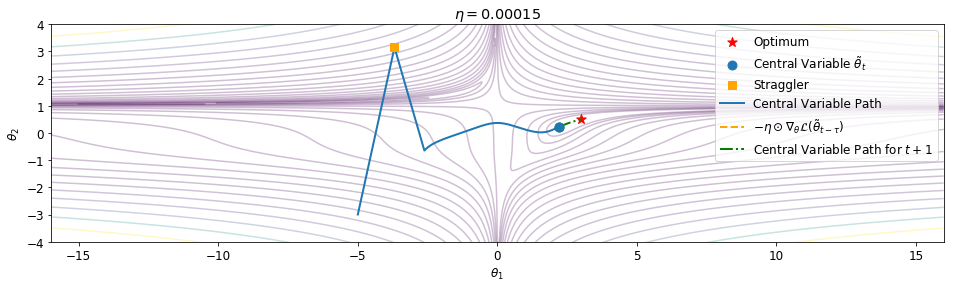
\includegraphics[width=\textwidth]{resources/images/async_straggler_corrected_adag}
  \caption{Correction of the stale worker delta using Equation~\ref{eq:adag}. Contrary to Figure~\ref{fig:async_momentum}, the gradient is scaled down significantly in a way it does not deteriorate the performance of the central variable.}
  \label{fig:adag_straggler_corrected}
\end{figure}

An interesting observation from Chapter~\ref{chapter:accumulated_gradient_normalization}, is that contrary to \textsc{agn}, \textsc{aeasgd} does not show any divergent behaviour for most configurations, i.e., in terms of distributed hyperparameterizations. This is rather interesting, because it tells us that \textsc{aeasgd} has an intrinsic mechanism to deal with parameter staleness. If we review Equation~\ref{eq:aeasgd_worker}, which describes the worker update rule for $\lambda = 1$, we see the that the elastic difference, defined as $\eta_t\rho(\theta^k_t - \tilde{\theta}_t)$, incorperates the \emph{distance} between the worker parameterization $\theta^k_t$ and the \emph{current} parameterization of the central variable $\tilde{\theta}_t$. \textsc{aeasgd} uses the elastic difference as an \emph{opposing force} of the worker exploration, meaning, it limits the amount of exploration that can be done. As a result, the elastic difference of \textsc{aeasgd} in effect limits the \emph{distance} that can be covered by the worker (unless the gradients suddenly become larger). As a result, \textsc{aeasgd} serves as additional evidence for our notion that staleness should be defined in terms of \emph{distance}, and not in terms of stale steps, as formalized in Defination~\ref{def:staleness}.

\begin{definition}{Staleness}
  \label{def:staleness}
  Given a parameterization for worker $k$ at time $t$, $\theta^k_t$, based on the central variable $\tilde{\theta}_{t - \tau}$ where $\tau$ is the number of stale steps, and a central variable at time $t$, $\tilde{\theta}_t$. Then, staleness is defined as the difference (distance) between $\tilde{\theta}_t$ and $\tilde{\theta}_{t-\tau}$.
\end{definition}

Using Definition~\ref{def:staleness}, we can make the deduction that staleness is not really a problem as long as workers commit gradients based on older parameterization of the central variable, which are close to the \emph{current} central variable. This is again additional support for Hypothesis~\ref{hyp:local_optimization}, which states that workers only contribute efficiently to the central variable as they remain close to each other, i.e., the variance of the workers amount the parameter space is small.

\section{Algorithm \& Update Rule}
\label{sec:adag_algorithm}

This Section fully describes the \textsc{adag} update rule, and several architectural decisions that can be made when implementing this technique. Furthermore, using Definition~\ref{def:staleness}, we show how \textsc{adag} can push the limits of asynchronous optimization further, while at the same time eliminating the need for (distributed) hyperparameter gridsearches to ensure convergence.\\

To describe the \textsc{adag} update rule, we use the same terminology and notation used in Definition~\ref{def:staleness} to further strengthen the intuition in parameter staleness, and how parameter staleness is used in Equation~\ref{eq:adag}. Let us consider the case when $\tau = 0$. In this situation, a worker $k$ computes the gradient based on $\tilde{\theta}_{t-\tau}$ which is equal to $\tilde{\theta}_t$. As a result, the distance between these two parameterizations will be 0, which results in the worker delta $\Delta\theta^k$ to be incorperated into the central variable \emph{as is}, and thereby causing the \textsc{adag} update rule to generalize to \textsc{sgd}. In the next step, we add more asynchronous workers to the optimization problem. By doing so, we implicitly increase the staleness as $\mathbf{E}[\tau] = (n - 1)$. As a result, parameter staleness in terms of stale steps, $\tau$, is expected to be larger than 0. Consequently, the distance between $\tilde{\theta}_t$ and $\tilde{\theta}_{t - \tau}$ is \emph{expected} to be non-zero causing the worker delta to be scaled down proportionally to the difference of these parameterizations. However, since parameter changes in Deep Learning usually consist of very small updates, we use the inverse learning rate ($\eta_t^{-1}$) to get a sense of the scale at which these updates operate at. Using the inverse learning rate in Equation~\ref{eq:adag}, and due to the fact that staleness (in terms of distance) is usually relatively small in Deep Learning since the gradients are scaled with respect to $\eta_t$, we find that \textsc{adag} scales the gradients more realistically. Since without the inverse learning rate, the scaling would be very small.

\begin{equation}
  \label{eq:adag}
  \tilde{\theta}_{t+1} = \tilde{\theta}_t + \ddfrac{1}{\eta_t^{-1}\|\tilde{\theta}_t - \tilde{\theta}_{t - \tau}\|^2 + 1} \odot \Delta\theta^k
\end{equation}

Nevertheless, one could view the inverse learning rate from a different perspective. Fist let us denote the set of workers as $\mathcal{W}$. Then, the staleness term in Equation~\ref{eq:adag} can be written as a sequence of gradients from different workers $w$, as shown in Equation~\ref{eq:adag_difference_1}.

\begin{equation}
  \label{eq:adag_difference_1}
  \tilde{\theta}_{t} - \tilde{\theta}_{t - \tau} = \sum_{i = 0}^\tau \exists!\, w \in \mathcal{W}: \eta_t \nabla_\theta \mathcal{L}_w(\tilde{\theta}_{t - \tau_w})
\end{equation}

Furthermore, assuming a static learning rate $\eta$, Equation~\ref{eq:adag_difference_1} can be simplified by moving the learning rate $\eta_t$ before the summation sign, obtaining Equation~\ref{eq:adag_difference_2}.

\begin{equation}
  \label{eq:adag_difference_2}
  \tilde{\theta}_{t} - \tilde{\theta}_{t - \tau} = \eta \sum_{i = 0}^\tau \exists!\, w \in \mathcal{W}: \nabla_\theta \mathcal{L}_w(\tilde{\theta}_{t - \tau_w})
\end{equation}

Remember that the scaling of the worker deltas are proportional to Equation~\ref{eq:adag_difference_3}.

\begin{equation}
  \label{eq:adag_difference_3}
  \eta^{-1} \|\tilde{\theta}_t - \tilde{\theta}_{t - \tau}\|^2
\end{equation}

Substituting the staleness term in Equation~\ref{eq:adag_difference_3} for Equation~\ref{eq:adag_difference_2} gives us:

\begin{equation}
  \label{eq:adag_difference_4}
  \eta^{-1}\|\eta\sum_{i = 0}^\tau \exists!\, w \in \mathcal{W}: \nabla_\theta \mathcal{L}_w(\tilde{\theta}_{t - \tau_w})\|^2
\end{equation}

Earlier, the assumption was made the learning rate is static. As a result, we can cancel the learning rate terms, and thus obtaining Equation~\ref{eq:adag_difference_5}.

\begin{equation}
  \label{eq:adag_difference_5}
  \cancel{\eta^{-1}}\|\cancel{\eta}\sum_{i = 0}^\tau \exists!\, w \in \mathcal{W}: \nabla_\theta \mathcal{L}_w(\tilde{\theta}_{t - \tau_w})\|^2
\end{equation}

This result indicates that the scaling term in Equation~\ref{eq:adag} is proportional to a \emph{unitless} sequence of worker gradients, i.e., not scaled down by a learning rate. As a result, Equation~\ref{eq:adag} is not sensitive to the hyperparameterization of $\eta$. Therefore, the scaling term will work at any scale, and still be proportional to the magnitude of the worker gradients.\\

An additional, but important aspect that needs to be considered is how \textsc{adag} keeps track of $\tilde{\theta}_{t - \tau}$. For this we foresee two possible implementations. The first, described in Algorithm~\ref{algo:adag_1}, keeps track of $\tilde{\theta}_{t - \tau_w}$ for a particular worker $w$ at a worker level. Meaning, worker $w$ keeps track of its local copy $\theta_t^w$, and the original central variable $\tilde{\theta}_{t-\tau}$. Next, when worker $w$ is done computing $\Delta\theta^w_t$, $w$ will commit both $\Delta\theta^w_t$ and $\tilde{\theta}_{t - \tau}$ to the parameter server. Since the parameter server already holds $\tilde{\theta}_{t}$, the parameter server can now compute the next central variable using Equation~\ref{eq:adag}.

\begin{algorithm}[H]
  \caption{Implementation of \textsc{adag} where the workers are responsible for keeping track of $\tilde{\theta}_{t - \tau}$.}
  \label{algo:adag_1}
  \begin{algorithmic}[1]
    \Procedure{ADAGParameterServer}{}
    \State $t \gets 0$ \Comment{Parameter server clock}
    \State $\tilde{\theta}_t \gets \Call{Random}$
    \State
    \Procedure{HandlePull}{$k$} \Comment{$k$ denotes the worker identifier}
    \State \Return $\tilde{\theta}_{t}$
    \EndProcedure
    \State
    \Procedure{HandleCommit}{$k$, $\Delta\theta^w$, $\tilde{\theta}_{t - \tau_k}$}
    \State $\tilde{\theta}_{t + 1} = \tilde{\theta}_t + \ddfrac{1}{\eta_t^{-1}\|\tilde{\theta}_t - \tilde{\theta}_{t - \tau_k}\|^2 + 1} \odot \Delta\theta^k_t$
    \State $t \gets t + 1$
    \EndProcedure
    \State
    \EndProcedure
  \end{algorithmic}
\end{algorithm}

However, an obvious limitation of Algorithm~\ref{algo:adag_1} is the increased network usage since two parameterizations have to be shipped to the parameter server, i.e., the worker delta $\Delta\theta^k_t$ and the original central variable parameterization $\tilde{\theta}_{t - \tau}$. To reduce the network usage of Algorithm~\ref{algo:adag_1}, and thereby reducing the waiting time of the workers, we propose to let the parameter server keep track of worker pulls, i.e., whenever a worker pulls the central variable, the parameter server copies the central variable into a datastructure (for example, a hashmap), and associates the the parameterization of the central variable with the worker which requested the pull at that time. This procedure is roughly described in Algorithm~\ref{algo:adag_2}. However, we would like to note that despite the fact that Algorithm~\ref{algo:adag_2} reduces the communication costs, it increases the memory requirements proportional to the number of concurrent workers, which might be problematic as the number of asynchronous workers is high.

\begin{algorithm}[H]
  \caption{Network efficient implementation of \textsc{adag}.}
  \label{algo:adag_2}
  \begin{algorithmic}[1]
    \Procedure{ADAGParameterServer}{}
    \State $t \gets 0$ \Comment{Parameter server clock}
    \State $\tilde{\theta}_t \gets \Call{Random}$
    \State $m \gets \Call{Initialize}$ \Comment{Initializes a data structure which keeps track of worker pulls.}
    \State
    \Procedure{HandlePull}{$k$} \Comment{$k$ denotes the worker identifier}
    \State $m[k] = \tilde{\theta}_t$
    \State \Return $\tilde{\theta}_{t}$
    \EndProcedure
    \State
    \Procedure{HandleCommit}{$k$, $\Delta\theta^w$}
    \State $\tilde{\theta}_{t + 1} = \tilde{\theta}_t + \ddfrac{1}{\eta_t^{-1}\|\tilde{\theta}_t - m[k]\|^2 + 1} \odot \Delta\theta^k_t$
    \State $t \gets t + 1$
    \EndProcedure
    \State
    \EndProcedure
  \end{algorithmic}
\end{algorithm}

However, there is a pratical problem in Algorithm~\ref{algo:adag_1} and Algorithm~\ref{algo:adag_2} which tends to be overlooking when viewing \textsc{adag} from a theoretical perspective. that is, both Algorithm~\ref{algo:adag_1} and Algorithm~\ref{algo:adag_2} put severe computational load on the parameter server to ensure consistency of the staleness computation when computing the scaling factor. Remember that in order to ensure staleness consistency, we lock any writes to the central variable during the time the parameter server computes the scaling factor. This induces a significant wait in other workers due to relatively heavy computations which need to be executed by the parameter server. However, taking inspiration from \textsc{aeasgd}~\cite{zhang2015deep}, we can make significant improvements regarding computationial efficiency if we loosen the consistency constraints. By doing so, we could let the workers compute the scaling factor locally, and then transmit the scaled delta to the parameter server which only has to \emph{add} the delta into the central variable. Furthermore, to reduce the network usage even more, we only pull the central variable only once, as shown in Algorithm~\ref{algo:adag_2}. Despite the fact that Algorithm~\ref{algo:adag_2} is more computationally efficient because the load is parallelized equally over all workers, it has several consistency issues. The first being that the computed scaling factor \emph{might} not reflect reality since other workers \emph{could} have committed their deltas to the parameter server between the time our worker pulled the central variable, and the committed its scaled delta. Furthermore, if this occurs, the worker will start computing gradients based on an already (slightly) stale central variable in the next iteration.

\begin{algorithm}[H]
  \caption{Network efficient, and more computational efficient implementation of \textsc{adag}. With the side-effect that we loosen the staleness consistency constraints.}
  \label{algo:adag_2}
  \begin{algorithmic}[1]
    \Procedure{ADAGWorker}{$k$}
    \State $\tilde{\theta}_\text{original} \gets \Call{Pull}$ \Comment{Keep a local copy of the central variable}
    \State $\theta^k_t \gets \tilde{\theta}_\text{original}$
    \State
    \Procedure{Commit}{$\Delta\theta^w$} \Comment{Redefine \textsc{Commit} operation.}
    \State $\tilde{\theta}_t \gets \Call{Pull}$
    \State $\Delta\theta^k \gets \ddfrac{1}{\eta_t^{-1}\|\tilde{\theta}_t - \tilde{\theta}_\text{original}|^2 + 1} \odot \Delta\theta^k$
    \State $\Call{SendToParameterServer}{\Delta\theta^k}$
    \State $\tilde{\theta}_\text{original} \gets \tilde{\theta}_t$
    \State $\theta^k_t \gets \tilde{\theta}_\text{original}$
    \State $t \gets t + 1$
    \EndProcedure
    \State
    \EndProcedure
  \end{algorithmic}
\end{algorithm}

\section{Experiments}
\label{sec:adag_experiments}

To demonstrate the effectiveness of Definition~\ref{def:staleness}, several experiments shall be conducted in the following section regarding the convergence properties of \textsc{adag}. Looking back at Chapter~\ref{chapter:accumulated_gradient_normalization}, we saw that staleness mitigation is critical in highly concurrent environments, as the staleness increases proportionally to the number of workers, as shown in Figure~\ref{fig:staleness_increasing}. Furthermore, without \textsc{adag}, we have to descrease the communication frequency even further to ensure that divergence does not occur. However, as a result of the increased amount of local exploration, parameter updates occur less frequently. Which again results in a slower convergence of the central variable, and thereby reducing the \emph{temporal efficiency} of those highly concurrent configurations compared to less concurrent configurations.\\

Let us start by considering several predictive scenarios to verify this novel understanding of parameter staleness in Deep Learning, and how to deal with it, as shown in Equation~\ref{eq:adag}. First and foremost, at the start of any parameterized machine learning training procedure, a model is initialized according to some initialization strategy. Since the probability is \emph{very} low that a randomly initialized parameterization will perform well in terms of classification accuracy, we can make the assumption that the loss during the initial phase of the training will be relatively high. Furthermore, let us assume that there are $n$ workers trying to optimize the central variable in an asynchronous manner, and that \textsc{adag} is applied before incorperating the worker deltas into the central variable, i.e., scaling proportional to $n^{-1}\|\tilde{\theta}_t - \tilde{\theta}_{t - \tau}\|^2$ is applied to the incoming worker delta. In this case, we can expect that during the initial phase of the training procedure only a few workers will contribute efficiently to the central variable. With this statement, we are implying that only the deltas of a small fraction of workers will not be scaled down significantly because the loss, and thereby the gradients are quite large at the start of the training procedure, in contrast to the situation when the central variable is close to an optimum. As a result, other workers will be scaled down significantly, because the parameterization on which they based their gradients on (which all workers started with), is too distant from the current central variable.

\begin{figure}[H]
  \centering
  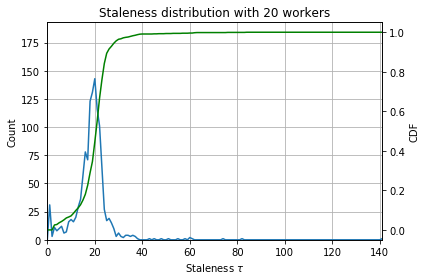
\includegraphics[width=.4\textwidth]{resources/images/plots/adag_agn_mnist/epoch_40/15/000000001/staleness_distribution}
  \caption{Staleness distribution of $n = 20$. This is in accordance with the theory~\cite{implicitmomentum}, which says that $\mathbf{E}[\tau] = (n - 1)$. Note that the $x$-axis denotes the staleness in terms of stale steps.}
  \label{fig:staleness_increasing}
\end{figure}

The following prediction we make is related to the convergence of optimizers which employ \textsc{adag}. First, we know that stale gradients will be scaled down significantly due to the update rule described in Equation~\ref{eq:adag}. Furthermore, since the loss is getting smaller as the training procedure goes on, staleness, in terms of Definition~\ref{def:staleness}, is implicitly getting smaller as well. As a result, if one would plot the scaling term for every worker, we should observe (on average) a decline in the scaling factor. This would imply that the distance between the central variables, and thereby the worker gradients are small. As a result, worker deltas do not have to be scaled down as much as their gradients are relatively local to the current central variable. Furthermore, in such a situation, the optimization process would benifit from more asynchronous workers since the staleness is relatively small. An additonal situation where more asynchronous workers would be benificial is on a \emph{plateau}, where the losses are very small which implies that the parameter updates are very small. In such a situation, \textsc{adag} would barely scale down the gradients. Furthermore, as the workers would ``leave'' the plateau, worker updates which are too stale would automatically be nullified.\\

To emperically validate these predictions, we conducted several experiments for which we know \textsc{agn} has difficulities converging, i.e., high amount of asynchrony and a high communication frequency. Furthermore, to show that Definition~\ref{def:staleness} is a better description of staleness compared to the number of steps, we will show that staleness, in number of steps, in not necessarily proportional to the scaling factor. This is a valid assumption to make since the scaling factor \emph{is} proportional to the distance between parameterizations.

\begin{figure}[H]
  \centering
  % So far for file naming consistency.
  \begin{subfigure}{.3\textwidth}
    \centering
    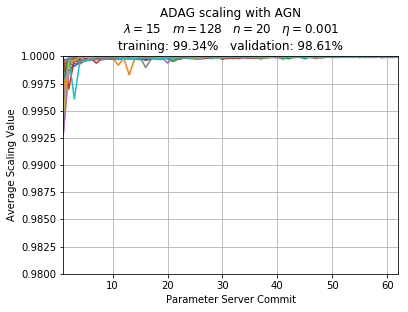
\includegraphics[width=\linewidth]{resources/images/plots/adag_agn_mnist/epoch_40/15/001/adag_agn_scaling_overview}
    \caption{$\eta = 0.001$}
  \end{subfigure}
  \begin{subfigure}{.3\textwidth}
    \centering
    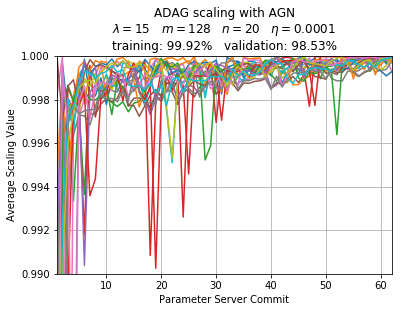
\includegraphics[width=\linewidth]{resources/images/plots/adag_agn_mnist/epoch_40/15/0001/scaling_detail}
    \caption{$\eta = 0.0001$}
  \end{subfigure}
  \begin{subfigure}{.3\textwidth}
    \centering
    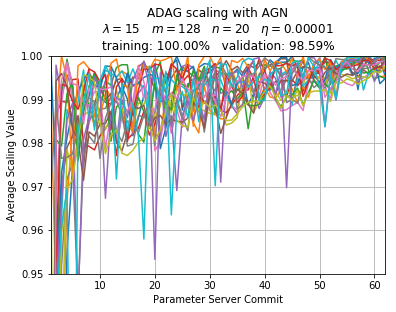
\includegraphics[width=\linewidth]{resources/images/plots/adag_agn_mnist/epoch_40/15/00001/scaling_overview}
    \caption{$\eta = 0.00001$}
  \end{subfigure}
  \caption{Average scaling (of all weights) value of every worker in \textsc{adag} with respect to different learning rates. In all Subfigures we observe a significant scaling at the start of the learning procedure (loss is relatively high, as mentioned in our first prediction), while at the end of the training procedure, scaling is not very prominent because the workers converged to a minima.}
  \label{fig:adag_predictions}
\end{figure}

\newpage
Figure~\ref{fig:adag_worker_staleness_and_scaling} shows the stale steps (top row), together with the average scaling factor (bottom row) of every worker. Since \textsc{adag} provides a per-weight scaling factor, we compute the average scaling factor by averaging all scaling factors for every trainable weight. This allows us to get a general overview of how the scaling term behaves under different values of staleness. Looking at Figure~\ref{fig:adag_worker_staleness_and_scaling}, we observe a significant scaling at the start of the optimization procedure \emph{for most workers}, thus providing evidence for our initial prediction. Furthermore, to show that the number of stale steps is not necessarily proportional to staleness in terms of distance, let us consider \emph{Worker 2} in Figure~\ref{fig:adag_worker_staleness_and_scaling} for a moment. Around parameter update step 12, a very stale update was committed to the parameter server, both in distance as in number of steps. However, other updates of \emph{Worker 2} are also quite stale compared to other workers. Yet, the scaling factor for these updates are almost equal to 0, thus indicating that the number of stale steps is not necessarily proportional to the real staleness. Of course, this begs the question why other workers for these particular update numbers have significantly lower scaling factors, while their staleness is lower as well. This can be explained by the fact that \emph{Worker 2} was significantly slower than other workers during the initial phase of the training procedure, which caused the central variable to have moved significantly towards a minima during that time. Of course, since gradients are relatively small in the neighbourhood of a minima, staleness is not actively playing a role a in the divergence of the central variable. As a result, worker gradients are not scaled down. This result can be validated by looking at \emph{Worker 8} as well, since Worker 8 behaves in a similar manner.\\

Furthermore, Figure~\ref{fig:adag_worker_staleness_and_scaling} can serve as additional validation for the statement made in~\cite{implicitmomentum}, which says that $\textbf{E}[\tau] = (n - 1)$. If we look at the average staleness of all workers, we can immediately see that the \emph{expected} staleness value of the optimization process is about 20, which is the number of workers used in that particular experiment.\\

Finally, we apply \textsc{adag} to solve the instability issues of \textsc{agn} in Chapter~\ref{chapter:accumulated_gradient_normalization} under highly concurrent conditions with high communication frequencies, i.e., high number of asynchronous workers with frequent parameter updates. As shown in Figure~\ref{fig:applying_adag}, we see that \textsc{agn} initially has some difficulities converging to a minima due to the increased amount of staleness and \emph{implicit momentum}~\cite{implicitmomentum}. However, when \textsc{adag} is applied, this instability is gone because \textsc{adag} scales down worker deltas proportional to the distance of the old, and current central variable.

\begin{figure}[H]
  \centering
  \begin{subfigure}{.49\textwidth}
    \centering
    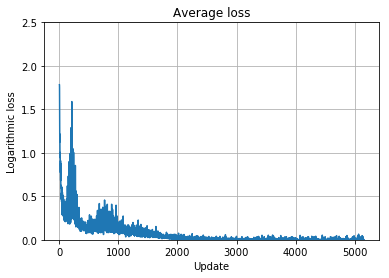
\includegraphics[width=\linewidth]{resources/images/adag_loss_original}
    \caption{\textsc{agn} without \textsc{adag}}
  \end{subfigure}
  \begin{subfigure}{.49\textwidth}
    \centering
    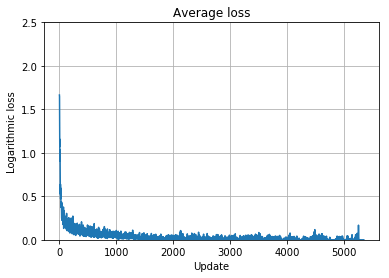
\includegraphics[width=\linewidth]{resources/images/adag_loss_corrected}
    \caption{\textsc{agn} with \textsc{adag}}
  \end{subfigure}
  \caption{In this experiment we apply \textsc{agn} to the MNIST problem using 30 asynchronous workers. From Subfigure (a) we observe some divergent behaviour of the central variable during the initial phase of the training procedure. However, if we apply \textsc{adag} to \textsc{agn} in these exact same conditions, the divergent behaviour previously observed is absent due to the fact that stale worker deltas are scaled down, or even nullified. Furthermore, since the divergent behaviour is not present in Subfigure (b), \textsc{agn} with \textsc{adag} reaches convergence faster (in terms of updates).}
  \label{fig:applying_adag}
\end{figure}

\begin{figure}
  \centering
  % Worker 1 till 4.
  \begin{subfigure}{.24\textwidth}
    \centering
    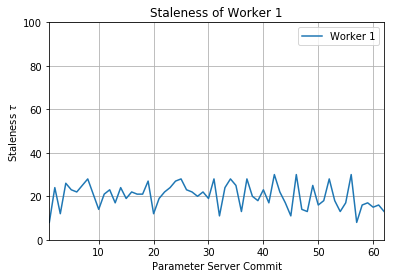
\includegraphics[width=\linewidth]{resources/images/plots/adag_agn_mnist/epoch_40/15/001/staleness/worker_1}
    \caption{Worker 1}
  \end{subfigure}
  \begin{subfigure}{.24\textwidth}
    \centering
    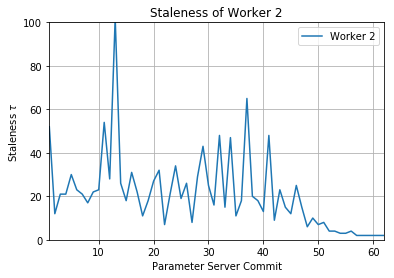
\includegraphics[width=\linewidth]{resources/images/plots/adag_agn_mnist/epoch_40/15/001/staleness/worker_2}
    \caption{Worker 2}
  \end{subfigure}
  \begin{subfigure}{.24\textwidth}
    \centering
    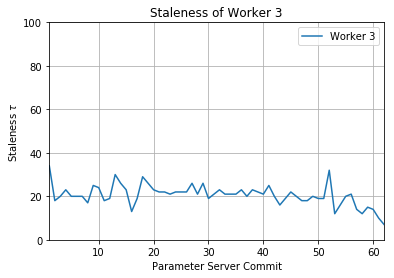
\includegraphics[width=\linewidth]{resources/images/plots/adag_agn_mnist/epoch_40/15/001/staleness/worker_3}
    \caption{Worker 3}
  \end{subfigure}
  \begin{subfigure}{.24\textwidth}
    \centering
    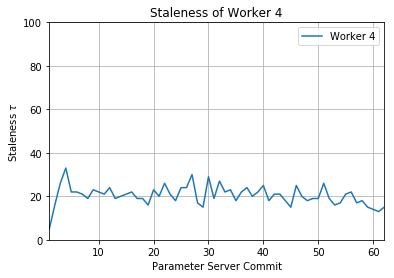
\includegraphics[width=\linewidth]{resources/images/plots/adag_agn_mnist/epoch_40/15/001/staleness/worker_4}
    \caption{Worker 4}
  \end{subfigure}
  % Scaling 1 till 4.
  \begin{subfigure}{.24\textwidth}
    \centering
    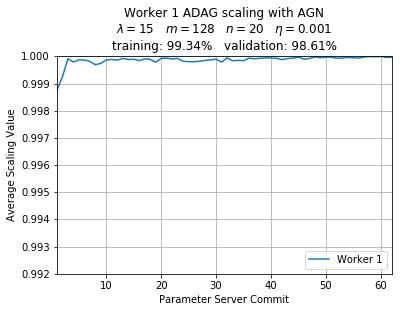
\includegraphics[width=\linewidth]{resources/images/plots/adag_agn_mnist/epoch_40/15/001/scaling/worker_1}
    \caption{Scaling worker 1}
  \end{subfigure}
  \begin{subfigure}{.24\textwidth}
    \centering
    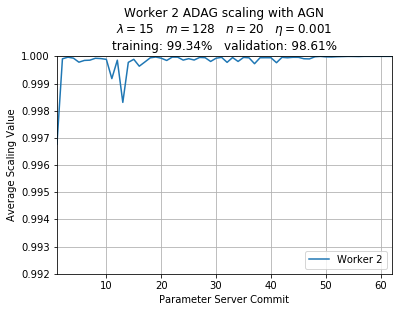
\includegraphics[width=\linewidth]{resources/images/plots/adag_agn_mnist/epoch_40/15/001/scaling/worker_2}
    \caption{Scaling worker 2}
  \end{subfigure}
  \begin{subfigure}{.24\textwidth}
    \centering
    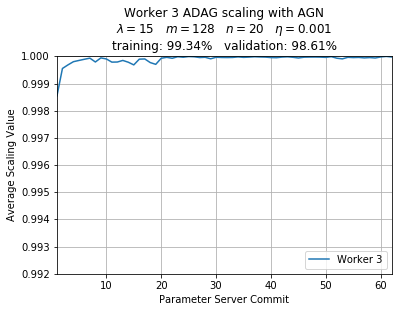
\includegraphics[width=\linewidth]{resources/images/plots/adag_agn_mnist/epoch_40/15/001/scaling/worker_3}
    \caption{Scaling worker 3}
  \end{subfigure}
  \begin{subfigure}{.24\textwidth}
    \centering
    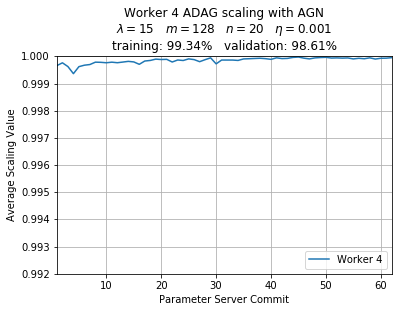
\includegraphics[width=\linewidth]{resources/images/plots/adag_agn_mnist/epoch_40/15/001/scaling/worker_4}
    \caption{Scaling worker 4}
  \end{subfigure}
  % Worker 5 till worker 8.
  \begin{subfigure}{.24\textwidth}
    \centering
    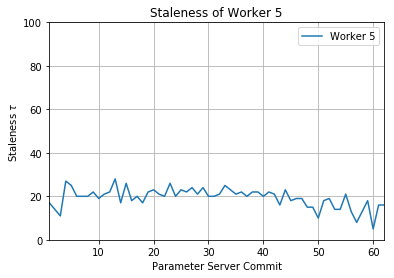
\includegraphics[width=\linewidth]{resources/images/plots/adag_agn_mnist/epoch_40/15/001/staleness/worker_5}
    \caption{Worker 5}
  \end{subfigure}
  \begin{subfigure}{.24\textwidth}
    \centering
    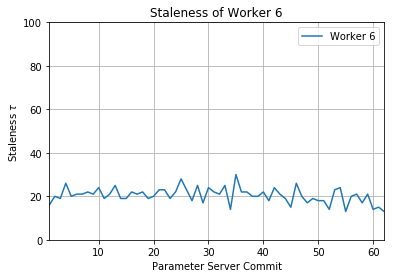
\includegraphics[width=\linewidth]{resources/images/plots/adag_agn_mnist/epoch_40/15/001/staleness/worker_6}
    \caption{Worker 6}
  \end{subfigure}
  \begin{subfigure}{.24\textwidth}
    \centering
    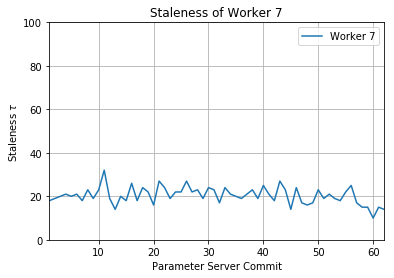
\includegraphics[width=\linewidth]{resources/images/plots/adag_agn_mnist/epoch_40/15/001/staleness/worker_7}
    \caption{Worker 7}
  \end{subfigure}
  \begin{subfigure}{.24\textwidth}
    \centering
    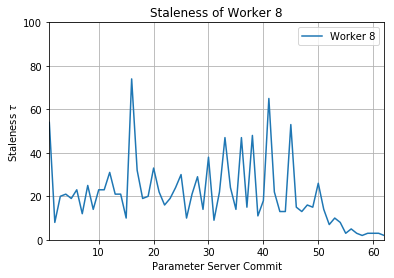
\includegraphics[width=\linewidth]{resources/images/plots/adag_agn_mnist/epoch_40/15/001/staleness/worker_8}
    \caption{Worker 8}
  \end{subfigure}
  % Scaling of worker 5 till worker 8.
  \begin{subfigure}{.24\textwidth}
    \centering
    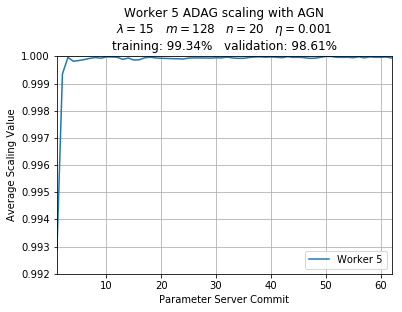
\includegraphics[width=\linewidth]{resources/images/plots/adag_agn_mnist/epoch_40/15/001/scaling/worker_5}
    \caption{Scaling worker 5}
  \end{subfigure}
  \begin{subfigure}{.24\textwidth}
    \centering
    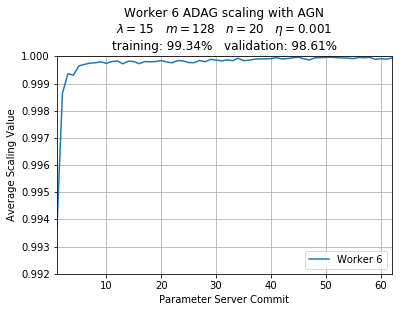
\includegraphics[width=\linewidth]{resources/images/plots/adag_agn_mnist/epoch_40/15/001/scaling/worker_6}
    \caption{Scaling worker 6}
  \end{subfigure}
  \begin{subfigure}{.24\textwidth}
    \centering
    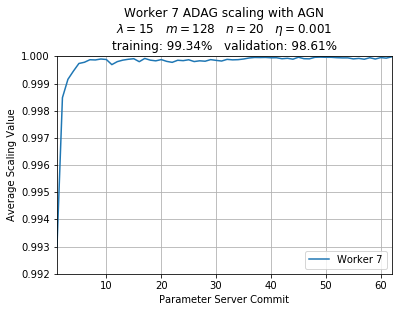
\includegraphics[width=\linewidth]{resources/images/plots/adag_agn_mnist/epoch_40/15/001/scaling/worker_7}
    \caption{Scaling worker 7}
  \end{subfigure}
  \begin{subfigure}{.24\textwidth}
    \centering
    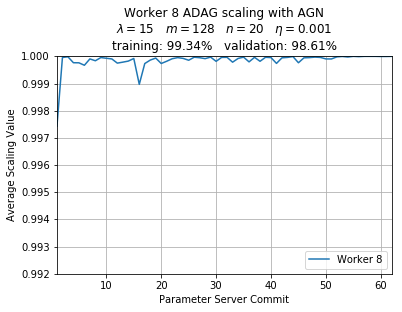
\includegraphics[width=\linewidth]{resources/images/plots/adag_agn_mnist/epoch_40/15/001/scaling/worker_8}
    \caption{Scaling worker 8}
  \end{subfigure}
  % Worker 9 till worker 12.
  \begin{subfigure}{.24\textwidth}
    \centering
    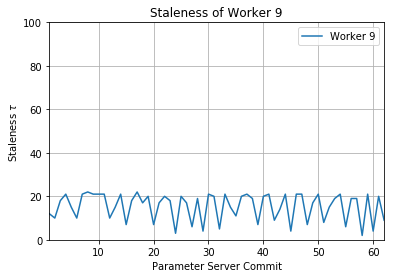
\includegraphics[width=\linewidth]{resources/images/plots/adag_agn_mnist/epoch_40/15/001/staleness/worker_9}
    \caption{Worker 9}
  \end{subfigure}
  \begin{subfigure}{.24\textwidth}
    \centering
    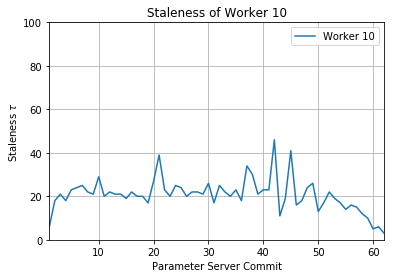
\includegraphics[width=\linewidth]{resources/images/plots/adag_agn_mnist/epoch_40/15/001/staleness/worker_10}
    \caption{Worker 10}
  \end{subfigure}
  \begin{subfigure}{.24\textwidth}
    \centering
    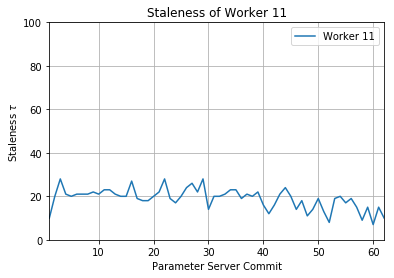
\includegraphics[width=\linewidth]{resources/images/plots/adag_agn_mnist/epoch_40/15/001/staleness/worker_11}
    \caption{Worker 11}
  \end{subfigure}
  \begin{subfigure}{.24\textwidth}
    \centering
    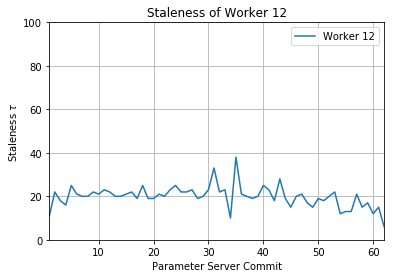
\includegraphics[width=\linewidth]{resources/images/plots/adag_agn_mnist/epoch_40/15/001/staleness/worker_12}
    \caption{Worker 12}
  \end{subfigure}
  % Scaling of worker 9 till worker 12.
  \begin{subfigure}{.24\textwidth}
    \centering
    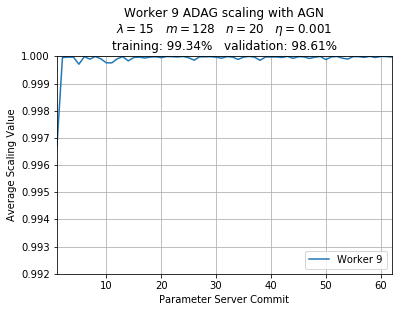
\includegraphics[width=\linewidth]{resources/images/plots/adag_agn_mnist/epoch_40/15/001/scaling/worker_9}
    \caption{Scaling worker 9}
  \end{subfigure}
  \begin{subfigure}{.24\textwidth}
    \centering
    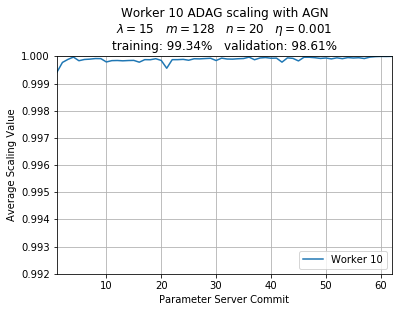
\includegraphics[width=\linewidth]{resources/images/plots/adag_agn_mnist/epoch_40/15/001/scaling/worker_10}
    \caption{Scaling worker 10}
  \end{subfigure}
  \begin{subfigure}{.24\textwidth}
    \centering
    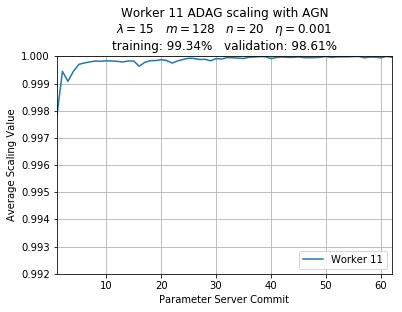
\includegraphics[width=\linewidth]{resources/images/plots/adag_agn_mnist/epoch_40/15/001/scaling/worker_11}
    \caption{Scaling worker 11}
  \end{subfigure}
  \begin{subfigure}{.24\textwidth}
    \centering
    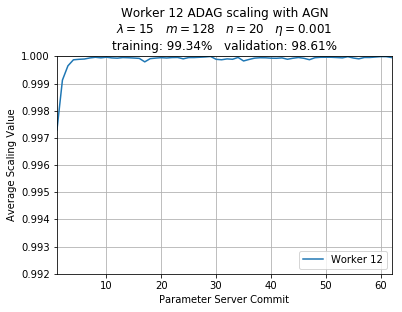
\includegraphics[width=\linewidth]{resources/images/plots/adag_agn_mnist/epoch_40/15/001/scaling/worker_12}
    \caption{Scaling worker 12}
  \end{subfigure}
  \caption{Worker staleness and scaling factor of Worker 1 till Worker 12. In the top row, we show the number of stale steps between every parameter update. Whereas in the bottom row, we show the scaling factor corresponding to the same parameter update step.}
  \label{fig:adag_worker_staleness_and_scaling}
\end{figure}

\section{Future work}
\label{sec:adag_future_work}
